\documentclass[11pt]{article}

\usepackage[margin=1in]{geometry}
\usepackage{amsmath}
\usepackage{amssymb}
\usepackage{xcolor}
\usepackage[most]{tcolorbox}
\usepackage{enumitem}
\usepackage{titlesec}
\usepackage{tikz}
\usepackage{hyperref}

% Links map to the structural header blue.
% bookmarks=false avoids the spaced-jobname .out failure on Windows/tectonic.
\hypersetup{colorlinks=true, linkcolor=headerblue, urlcolor=headerblue, bookmarks=false}

\tcbuselibrary{skins}

% 1.1 Palette
\definecolor{headerblue}{HTML}{1C569E}
\definecolor{accentgreen}{HTML}{2E7D32}
\definecolor{accentorange}{HTML}{E27A1E}
\definecolor{workpurple}{HTML}{A020F0}
\definecolor{warnred}{HTML}{C0392B}

% 1.2 Subsection Typography
\titleformat{\subsection}
  {\normalfont\large\bfseries\color{headerblue}}{\thesubsection}{1em}{}

% 2. Table of Contents Depth
\setcounter{secnumdepth}{2}
\setcounter{tocdepth}{2}

% 3. Box System (Unbreakable)
\newtcolorbox{topicsbox}{
    enhanced,
    colback=headerblue!6!white, colframe=headerblue,
    coltitle=white, fonttitle=\bfseries,
    title={Chapter 6 at a Glance: Switches, Spikes, and Impulse Forcing},
    boxrule=0.6pt, arc=2mm,
    left=3mm, right=3mm, top=2mm, bottom=2mm
}

\newtcolorbox{formulabox}[1][Master Formula]{
    enhanced,
    colback=accentorange!8!white, colframe=accentorange,
    coltitle=white, fonttitle=\bfseries,
    title={#1},
    boxrule=0.6pt, arc=1mm,
    left=3mm, right=3mm, top=2mm, bottom=2mm
}

\newtcolorbox{methodbox}[1][Method]{
    enhanced,
    colback=accentgreen!6!white, colframe=accentgreen,
    coltitle=white, fonttitle=\bfseries,
    title={#1},
    boxrule=0.6pt, arc=1mm,
    left=3mm, right=3mm, top=2mm, bottom=2mm
}

\newtcolorbox{examplebox}[1][Worked Example]{
    enhanced,
    colback=workpurple!4!white, colframe=workpurple,
    coltitle=white, fonttitle=\bfseries,
    title={#1},
    boxrule=0.4pt, sharp corners,
    borderline west={3pt}{0pt}{workpurple},
    left=5mm, right=3mm, top=2mm, bottom=2mm
}

\newtcolorbox{conceptbox}[1][Key Takeaway]{
    enhanced,
    colback=accentorange!5!white, colframe=accentorange,
    coltitle=white, fonttitle=\bfseries,
    title={#1},
    boxrule=0.3pt, arc=1mm,
    left=3mm, right=3mm, top=2mm, bottom=2mm
}

\newtcolorbox{warningbox}[1][Common Pitfall]{
    enhanced,
    colback=red!3!white, colframe=warnred,
    coltitle=white, fonttitle=\bfseries,
    title={#1},
    boxrule=0.4pt, sharp corners,
    borderline west={3pt}{0pt}{warnred},
    left=5mm, right=3mm, top=2mm, bottom=2mm
}

\begin{document}

\begin{center}
    {\Large\bfseries\color{headerblue} Heaviside Step Functions, Dirac Delta,\\[2pt] and Impulse Forcing}\\[6pt]
    \large Chapter 6 --- A Self-Study Reference \& Master Guide\\[2pt]
    \normalsize\itshape A Math Confidence Reset
\end{center}
\vspace{0.4cm}

\tableofcontents
\vspace{0.8cm}

%======================================================================
\phantomsection
\addcontentsline{toc}{section}{Part I --- Theory \& Worked Examples}
\section*{Part I --- Theory \& Worked Examples}
\setcounter{section}{3}
\setcounter{subsection}{3}

\begin{topicsbox}
\begin{itemize}[leftmargin=*, itemsep=2pt]
  \item \textbf{The Heaviside Step Function (3.4):} a mathematical ``switch.'' The unit step $u_a(t)$ is $0$ before $t = a$ and $1$ after, so multiplying by it turns a term \emph{on} at a chosen instant. It is the language for forcing that arrives, departs, or changes abruptly --- and the Second Shift Theorem $\mathcal{L}\{u_a(t)f(t-a)\} = e^{-as}F(s)$ is the gear that moves it through the transform.
  \item \textbf{The Dirac Delta Function (3.5):} an idealized ``spike.'' Built as the limit of a tall, thin rectangular pulse of fixed area $1$, $\delta(t-t_0)$ models an instantaneous kick --- a hammer blow, a current surge, a sudden push. Its sifting property samples a function at a single point, and its transform is the strikingly clean $\mathcal{L}\{\delta(t-t_0)\} = e^{-st_0}$.
  \item \textbf{Why they belong together:} the delta is the \emph{derivative} of the step. A switch flipped infinitely fast \emph{is} an impulse. Together they let Laplace methods handle forcing that classical $e^{rt}$ guessing cannot touch.
\end{itemize}
\end{topicsbox}

\subsection{The Heaviside Step Function --- Mathematics as a Switch}

Up to now every forcing function $g(t)$ on the right-hand side of $a y'' + b y' + c y = g(t)$ has been a single smooth formula valid for all time: a polynomial, an exponential, a sinusoid. Real systems are not so polite. A voltage is applied at $t = 7$ seconds and not before. A load is dropped onto a beam and then removed. A thermostat clicks on. These are \emph{switches}, and to write them as one honest formula we need a function that is genuinely off, then genuinely on.

\subsubsection*{Historical Context: Oliver Heaviside and the Operational Calculus}

Before this machinery existed, engineers solving circuit problems faced a real struggle. Forcing that ``switched on'' had to be handled by splitting time into intervals, solving the differential equation separately on each piece, and then painstakingly matching the solution and its derivative at every junction so the pieces glued together continuously. The bookkeeping was brutal and error-prone, and it obscured the physics.

Oliver Heaviside (1850--1925), a self-taught English telegraph engineer and physicist, changed this. Working on signal propagation in undersea cables, he developed what he called the \emph{operational calculus}: he treated the differentiation symbol $p = \frac{d}{dt}$ as if it were an ordinary algebraic quantity, turning differential equations into algebra he could manipulate directly. His unit step --- the function that is $0$ until a chosen instant and $1$ thereafter --- gave him a clean symbol for ``the switch closes now.''

Heaviside's methods \emph{worked}, spectacularly, but he could not rigorously justify why, and the mathematical establishment of his day dismissed his manipulations as reckless. (``Mathematics is an experimental science,'' he retorted, ``and definitions do not come first, but later on.'') Vindication came afterward: the Laplace transform supplied exactly the rigorous foundation his operational calculus had been reaching for. The transform variable $s$ is the legitimate, fully justified version of Heaviside's bold symbol $p$, and the step function that bears his name is now a cornerstone of engineering mathematics.

\subsubsection*{Definition and the Shifted Step}

\begin{formulabox}[The Unit Step (Heaviside) Function]
The \textbf{unit step} switched on at $t = a \ge 0$ is
\[ u_a(t) \;=\; u(t-a) \;=\;
   \begin{cases}
     0, & t < a,\\[2pt]
     1, & t \ge a.
   \end{cases} \]
It is $0$ before the switch and $1$ after. The basic transform follows directly from the definition:
\[ \mathcal{L}\{u_a(t)\} = \int_{a}^{\infty} e^{-st}\,dt = \frac{e^{-as}}{s}, \qquad s > 0. \]
\end{formulabox}

The integral above starts at $t = a$ rather than $0$ because the integrand $e^{-st}u_a(t)$ is zero on $[0,a)$ --- the switch contributes nothing there. Evaluating, $\int_a^\infty e^{-st}\,dt = \left[-\tfrac1s e^{-st}\right]_a^\infty = \tfrac1s e^{-as}$, since $e^{-st} \to 0$ as $t \to \infty$.

\begin{center}
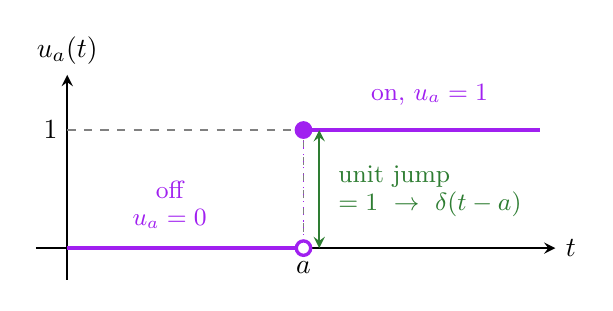
\begin{tikzpicture}[>=stealth, scale=1.0]
  % axes
  \draw[->, thick] (-0.4,0) -- (6.2,0) node[right] {$t$};
  \draw[->, thick] (0,-0.4) -- (0,2.2) node[above] {$u_a(t)$};
  % tick at a
  \draw[dashed, gray] (3,0) -- (3,1.5);
  \node[below] at (3,-0.05) {$a$};
  \node[left] at (0,1.5) {$1$};
  \draw[dashed, gray] (0,1.5) -- (3,1.5);
  % the step: 0 on [0,a), 1 on [a,inf)
  \draw[very thick, workpurple] (0,0) -- (3,0);
  \draw[very thick, workpurple] (3,1.5) -- (6,1.5);
  % jump indicator
  \draw[dotted, workpurple] (3,0) -- (3,1.5);
  % unit-jump dimension arrow (the "rise"), tying the step to the delta
  \draw[<->, thick, accentgreen] (3.2,0) -- (3.2,1.5);
  \node[accentgreen, align=left, right] at (3.32,0.72) {\small unit jump\\[-2pt]\small $= 1\ \to\ \delta(t-a)$};
  % open circle at (a,0), closed at (a,1)
  \filldraw[fill=white, draw=workpurple, very thick] (3,0) circle (2.6pt);
  \filldraw[fill=workpurple, draw=workpurple, very thick] (3,1.5) circle (2.6pt);
  \node[workpurple, align=center] at (1.3,0.55) {\small off\\[-2pt]\small $u_a = 0$};
  \node[workpurple, align=center] at (4.6,1.95) {\small on, $u_a = 1$};
\end{tikzpicture}
\end{center}
\begin{center}
\small\itshape The unit step $u_a(t)$: a clean jump discontinuity at $t = a$, rising by exactly $1$. That ``unit jump'' is the visceral link to the next section --- compressing this entire rise into an instant is precisely what makes its derivative the unit-area Dirac delta, $\frac{d}{dt}u_a(t) = \delta(t - a)$. Open circle = value not attained; filled circle = value attained.
\end{center}

\subsubsection*{Encoding Piecewise Functions}

Steps are the alphabet for piecewise forcing. Two patterns cover almost everything:

\begin{itemize}[leftmargin=*, itemsep=3pt]
  \item \textbf{Turn a term on at $t = a$:} multiply it by $u_a(t)$. The product $u_a(t)\,g(t)$ is $0$ until $a$, then $g(t)$.
  \item \textbf{A finite ``window'' on $[a,b)$:} subtract two steps, $u_a(t) - u_b(t)$. This is $1$ only on $[a,b)$ and $0$ elsewhere --- an on/off gate.
\end{itemize}

For instance, a forcing that holds the constant value $5$ until $t = 7$ and then shuts off is exactly $5\big(1 - u_7(t)\big)$: it equals $5$ on $[0,7)$ and $0$ for $t \ge 7$. That is precisely the forcing in the worked example below.

\subsubsection*{The Second Shift Theorem --- Moving a Switch Through the Transform}

To \emph{solve} equations with step forcing we need to know how a delayed, switched-on function transforms. The answer is the Second Shift Theorem (also called the $t$-shift or time-delay theorem).

\begin{formulabox}[Second Shift Theorem (Time Delay)]
If $\mathcal{L}\{f(t)\} = F(s)$, then a copy of $f$ delayed to start at $t = a$ and switched on there satisfies
\[ \mathcal{L}\big\{\,u_a(t)\,f(t-a)\,\big\} = e^{-as}\,F(s). \]
Read in reverse --- the form we use to \emph{invert} --- it says
\[ \mathcal{L}^{-1}\big\{\,e^{-as}\,F(s)\,\big\} = u_a(t)\,f(t-a), \qquad\text{where } f = \mathcal{L}^{-1}\{F\}. \]
\end{formulabox}

The structure to internalize: an exponential factor $e^{-as}$ in the $s$-domain is a \emph{time delay} of $a$ in the $t$-domain. When you spot $e^{-as}$ multiplying some transform $F(s)$, the inverse is the ordinary inverse of $F$ --- call it $f(t)$ --- with two non-negotiable modifications: (1) every $t$ becomes $t - a$, and (2) the whole thing is gated by $u_a(t)$. Skip either and the answer is wrong.

\begin{examplebox}[Worked Example 1: Solving an ODE with Discontinuous Forcing]
Solve the driven, damped oscillator
\[ y'' + 2y' + 5y = h(t), \qquad h(t) = 5\big(1 - u_7(t)\big), \qquad y(0) = 0,\ y'(0) = 0. \]
Physically: a constant drive of strength $5$ acts from $t = 0$, then is switched off abruptly at $t = 7$. We start from rest ($y(0) = y'(0) = 0$).

\smallskip
\textbf{Step 1 --- Transform the forcing.} Write $h(t) = 5 - 5u_7(t)$. Using $\mathcal{L}\{1\} = \tfrac1s$ and $\mathcal{L}\{u_7(t)\} = \tfrac{e^{-7s}}{s}$,
\[ \color{workpurple} \mathcal{L}\{h(t)\} = \frac{5}{s} - \frac{5e^{-7s}}{s}. \]

\textbf{Step 2 --- Transform the equation.} With zero initial conditions, $\mathcal{L}\{y''\} = s^2 Y$ and $\mathcal{L}\{y'\} = sY$, so
\[ \color{workpurple} (s^2 + 2s + 5)\,Y(s) = \frac{5}{s} - \frac{5e^{-7s}}{s}. \]

\textbf{Step 3 --- Isolate $Y(s)$.} Divide through by $s^2 + 2s + 5$:
\[ \color{workpurple} Y(s) = \frac{5}{s(s^2 + 2s + 5)} \;-\; e^{-7s}\,\frac{5}{s(s^2 + 2s + 5)}. \]
Both terms share the same core transform $F(s) = \dfrac{5}{s(s^2 + 2s + 5)}$; the second simply carries the delay factor $e^{-7s}$. Invert $F$ once and reuse it.

\smallskip
\textbf{Step 4 --- Partial fraction decomposition of $F(s)$.} The denominator has a simple root at $s = 0$ and an irreducible quadratic, so set up
\[ \color{workpurple} \frac{5}{s(s^2 + 2s + 5)} = \frac{A}{s} + \frac{Bs + C}{s^2 + 2s + 5}. \]
Clear denominators by multiplying both sides by $s(s^2+2s+5)$:
\[ \color{workpurple} 5 = A(s^2 + 2s + 5) + (Bs + C)\,s = (A + B)s^2 + (2A + C)s + 5A. \]
Match coefficients of like powers of $s$ on the two sides:
\[ \color{workpurple}
   \underbrace{5A = 5}_{s^0}, \qquad
   \underbrace{2A + C = 0}_{s^1}, \qquad
   \underbrace{A + B = 0}_{s^2}. \]
From the first, $A = 1$. Then $B = -A = -1$, and $C = -2A = -2$. Hence
\[ \color{workpurple} F(s) = \frac{1}{s} + \frac{-s - 2}{s^2 + 2s + 5}. \]
\end{examplebox}

\begin{examplebox}[Worked Example 1, continued: Inversion and Reassembly]
Recall the split transform $Y(s) = F(s) - e^{-7s}F(s)$ with $F(s) = \dfrac{1}{s} + \dfrac{-s-2}{s^2 + 2s + 5}$ from the decomposition above.

\smallskip
\textbf{Step 5 --- Complete the square and split for inversion.} Write $s^2 + 2s + 5 = (s+1)^2 + 2^2$. To match the shifted sine/cosine forms we re-express the numerator in terms of $(s+1)$:
\[ \color{workpurple} -s - 2 = -(s + 1) - 1, \]
so that
\[ \color{workpurple} \frac{-s-2}{(s+1)^2 + 4} = -\,\frac{s+1}{(s+1)^2 + 4} \;-\; \frac{1}{2}\cdot\frac{2}{(s+1)^2 + 4}. \]
The last term was multiplied and divided by $2$ so its numerator matches the standard form $\dfrac{2}{(s+1)^2 + 2^2} \to e^{-t}\sin(2t)$.

\smallskip
\textbf{Step 6 --- Invert to get the core response $f(t)$.} Using $\mathcal{L}^{-1}\{\tfrac1s\} = 1$, the $s$-shift rule $\mathcal{L}^{-1}\{\frac{s+1}{(s+1)^2+4}\} = e^{-t}\cos 2t$, and $\mathcal{L}^{-1}\{\frac{2}{(s+1)^2+4}\} = e^{-t}\sin 2t$:
\[ \color{workpurple} f(t) = \mathcal{L}^{-1}\{F(s)\} = 1 - e^{-t}\cos 2t - \tfrac{1}{2}e^{-t}\sin 2t. \]

\textbf{Step 7 --- Reassemble with the time delay.} Now invert $Y(s) = F(s) - e^{-7s}F(s)$. The first piece inverts to $f(t)$. The second carries $e^{-7s}$, so by the Second Shift Theorem it inverts to $u_7(t)\,f(t-7)$:
\[ \color{workpurple} y(t) = f(t) - u_7(t)\,f(t - 7). \]
Writing $f(t-7)$ explicitly --- every $t$ replaced by $t - 7$ --- gives the final answer:
\[ \color{workpurple}
   y(t) = \Big[\,1 - e^{-t}\cos 2t - \tfrac{1}{2}e^{-t}\sin 2t\,\Big]
        - u_7(t)\Big[\,1 - e^{-(t-7)}\cos 2(t-7) - \tfrac{1}{2}e^{-(t-7)}\sin 2(t-7)\,\Big]. \]
For $t < 7$ the gate $u_7$ is off and the system rings down toward the steady value $1$ under the constant drive; at $t = 7$ the drive cuts out and the second bracket switches on, steering the response back toward $0$.
\end{examplebox}

\begin{warningbox}[Forgetting the $u_a$ Factor]
When you invert a term carrying $e^{-as}$, the delay produces \textbf{two} effects, and beginners routinely apply only the first:
\begin{enumerate}[leftmargin=*, itemsep=1pt]
  \item Replace every $t$ by $t - a$ inside the function. \emph{(Usually remembered.)}
  \item Multiply the entire shifted function by the gate $u_a(t)$. \emph{(Frequently dropped.)}
\end{enumerate}
Writing $\mathcal{L}^{-1}\{e^{-7s}F(s)\} = f(t-7)$ \textbf{without} the $u_7(t)$ factor is wrong: that bare expression is nonzero for $t < 7$, claiming the delayed response acts \emph{before} it was triggered. The $u_a(t)$ is what enforces causality --- nothing happens until the switch is thrown. \textbf{Always carry the gate:} $\mathcal{L}^{-1}\{e^{-7s}F(s)\} = u_7(t)\,f(t-7)$.
\end{warningbox}

\begin{formulabox}[Exam Safeguard: Shifted Step vs.\ Delayed Function]
When $e^{-as}$ appears, decide \emph{what} it multiplies. A bare $e^{-as}/s$ is just the switch; an $e^{-as}F(s)$ is a whole function delayed --- and inverting it \textbf{must} restore the $u_a(t)$ gate.

\smallskip
\renewcommand{\arraystretch}{1.5}
\noindent\begin{tabular}{@{}p{0.30\linewidth}p{0.32\linewidth}p{0.30\linewidth}@{}}
\textbf{Object} & \textbf{Time domain} & \textbf{Transform / Inverse}\\[2pt]
\hline
Shifted step (switch alone) & $u_a(t)$ & $\mathcal{L}\{u_a(t)\} = \dfrac{e^{-as}}{s}$\\
Delayed function (forward) & $u_a(t)\,f(t-a)$ & $\mathcal{L}\{\cdot\} = e^{-as}F(s)$\\
Inverting $e^{-as}F(s)$ \textbf{(correct)} & $\textcolor{accentgreen}{u_a(t)}\,f(t-a)$ & $\mathcal{L}^{-1}\{e^{-as}F(s)\}$\\
Gate dropped \textbf{(wrong)} & \textcolor{warnred}{$f(t-a)$ alone} & --- acts before $t=a$\\
\hline
\end{tabular}

\smallskip
\textbf{Reading rule:} shift the argument $t \to t-a$ \emph{and} multiply by $u_a(t)$. The $\tfrac{1}{s}$ in the first row is special to the step itself; a general $F(s)$ keeps its own inverse $f$.
\end{formulabox}

\begin{conceptbox}[Key Takeaway]
The step function $u_a(t)$ is a \textcolor{accentorange}{switch}; the Second Shift Theorem $\mathcal{L}\{u_a(t)f(t-a)\} = e^{-as}F(s)$ is how that switch travels through the transform. An \textcolor{accentorange}{$e^{-as}$ in the $s$-domain always means a delay of $a$ in time} --- invert the bare transform, shift $t \to t - a$, and gate with $u_a(t)$.
\end{conceptbox}

\subsection{The Dirac Delta Function --- The Mathematics of an Instant}

A hammer strikes a bell. A bat meets a ball. A capacitor dumps its charge in a spark. In each case an enormous force acts over a vanishingly short time, and what the system ``feels'' is not the force at any instant but its accumulated effect --- the total impulse. We want an idealized object that captures ``a unit of push delivered all at once, at a single instant $t_0$.'' That object is the Dirac delta function, $\delta(t - t_0)$.

\subsubsection*{A Rigorous Foundation: the Limit of a Rectangular Pulse}

No ordinary function can be zero everywhere except at one point and still enclose a nonzero area --- a single point has zero width. So $\delta$ is not a function in the classical sense; it is a \emph{generalized function} (or \emph{distribution}), and the honest way to define it is as a \textbf{limit of ordinary functions} whose area is pinned at $1$ the entire way.

Center a rectangular pulse of width $2\alpha$ at $t_0$ using a symmetric (centered) difference of two steps:
\[ \delta_\alpha(t) = \frac{1}{2\alpha}\big[\,u_{t_0 - \alpha}(t) - u_{t_0 + \alpha}(t)\,\big]. \]
The bracket is the gate that is $1$ only on the interval $(t_0 - \alpha,\ t_0 + \alpha)$, of width $2\alpha$. Dividing by $2\alpha$ sets the height to $\tfrac{1}{2\alpha}$, so the enclosed area is
\[ \text{area} = \underbrace{2\alpha}_{\text{width}} \times \underbrace{\frac{1}{2\alpha}}_{\text{height}} = 1 \qquad\text{for every } \alpha > 0. \]
Now shrink the width: as $\alpha \to 0^{+}$ the pulse grows taller and narrower, but its area stays exactly $1$. The Dirac delta is the limiting object,
\[ \delta(t - t_0) = \lim_{\alpha \to 0^{+}} \frac{1}{2\alpha}\big[\,u_{t_0 - \alpha}(t) - u_{t_0 + \alpha}(t)\,\big], \]
characterized by being $0$ for all $t \ne t_0$ while carrying unit area concentrated at $t_0$.

\begin{center}
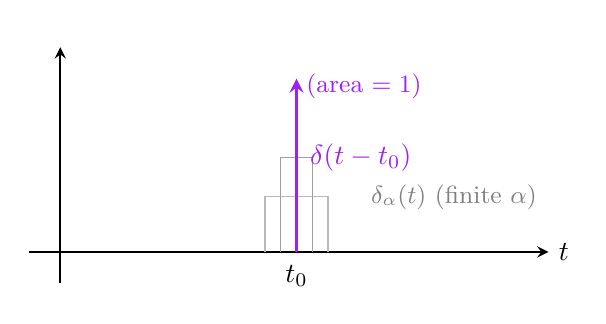
\begin{tikzpicture}[>=stealth, scale=1.0]
  % axes
  \draw[->, thick] (-0.4,0) -- (6.2,0) node[right] {$t$};
  \draw[->, thick] (0,-0.4) -- (0,2.6) node[above] {};
  % faint pre-limit pulses
  \draw[gray!55, thin] (2.6,0) -- (2.6,0.7) -- (3.4,0.7) -- (3.4,0);
  \draw[gray!75, thin] (2.8,0) -- (2.8,1.2) -- (3.2,1.2) -- (3.2,0);
  \node[gray] at (5.0,0.7) {\small $\delta_\alpha(t)$ (finite $\alpha$)};
  % the arrow = delta
  \draw[->, very thick, workpurple] (3,0) -- (3,2.2);
  \node[below] at (3,-0.05) {$t_0$};
  \node[workpurple, right] at (3,2.1) {\small (area $= 1$)};
  \node[workpurple, right] at (3.05,1.2) {$\delta(t - t_0)$};
\end{tikzpicture}
\end{center}
\begin{center}
\small\itshape The Dirac delta drawn as a vertical arrow at $t_0$. The arrow's \emph{height} is symbolic; the meaningful quantity is the enclosed \emph{area} $1$, the limit of the shrinking unit-area pulses (faint).
\end{center}

\subsubsection*{The Sifting Property}

The single most important fact about $\delta$ is how it behaves \emph{inside an integral} against a continuous test function $g$. It ``sifts out'' the value of $g$ at the spike.

\begin{formulabox}[The Sifting Property]
For any function $g$ continuous at $t_0$,
\[ \int_{-\infty}^{\infty} \delta(t - t_0)\,g(t)\,dt = g(t_0). \]
The delta acts as a sampling device: integrate any function against $\delta(t-t_0)$ and you read off that function's value at the single point $t_0$.
\end{formulabox}

\textbf{Proof (via the pulse limit).} Replace $\delta$ by the pre-limit pulse $\delta_\alpha$ and integrate. Because $\delta_\alpha$ is $\tfrac{1}{2\alpha}$ on $(t_0 - \alpha,\ t_0 + \alpha)$ and $0$ elsewhere, the infinite integral collapses to that short interval:
\[ \int_{-\infty}^{\infty} \delta_\alpha(t)\,g(t)\,dt = \frac{1}{2\alpha}\int_{t_0 - \alpha}^{\,t_0 + \alpha} g(t)\,dt. \]
The right side is exactly the \emph{average value} of $g$ over the interval $[t_0 - \alpha,\ t_0 + \alpha]$ (its integral divided by its length $2\alpha$). By the Mean Value Theorem for integrals, since $g$ is continuous there exists a point $c_\alpha \in (t_0 - \alpha,\ t_0 + \alpha)$ with
\[ \frac{1}{2\alpha}\int_{t_0 - \alpha}^{\,t_0 + \alpha} g(t)\,dt = g(c_\alpha). \]
As $\alpha \to 0^{+}$, the interval shrinks to the single point $t_0$, forcing $c_\alpha \to t_0$, and by continuity $g(c_\alpha) \to g(t_0)$. Therefore
\[ \int_{-\infty}^{\infty} \delta(t - t_0)\,g(t)\,dt = \lim_{\alpha \to 0^{+}} g(c_\alpha) = g(t_0). \qquad\blacksquare \]

\subsubsection*{The Laplace Transform of the Delta}

The transform now falls out of sifting in one line. Take $g(t) = e^{-st}$, which is continuous, and recall $t_0 \ge 0$:
\[ \mathcal{L}\{\delta(t - t_0)\} = \int_{0}^{\infty} e^{-st}\,\delta(t - t_0)\,dt = e^{-st}\Big|_{t = t_0} = e^{-s t_0}. \]

\begin{formulabox}[Transform of the Impulse]
\[ \mathcal{L}\{\delta(t - t_0)\} = e^{-s t_0}, \qquad\text{and in particular}\qquad \mathcal{L}\{\delta(t)\} = e^{0} = 1. \]
\end{formulabox}

This is remarkable: the impulse at the origin transforms to the constant $1$, the simplest object in the $s$-domain. An idealized kick excites the system across \emph{all} frequencies equally, which is exactly why $\mathcal{L}^{-1}\{1\} = \delta(t)$ and why striking a system with $\delta$ reveals its natural response.

\begin{examplebox}[Worked Example 2: The Hammer Strike]
Solve the damped oscillator struck by a unit impulse at $t = 4$:
\[ y'' + 2y' + 26y = \delta(t - 4), \qquad y(0) = 1,\ y'(0) = 0. \]
The system already sits displaced ($y(0) = 1$) and at rest ($y'(0) = 0$); at $t = 4$ a hammer delivers a unit impulse.

\smallskip
\textbf{Step 1 --- Transform each term, keeping the initial data.} Using $\mathcal{L}\{y''\} = s^2 Y - s\,y(0) - y'(0)$ and $\mathcal{L}\{y'\} = sY - y(0)$, with $y(0) = 1,\ y'(0) = 0$, and $\mathcal{L}\{\delta(t-4)\} = e^{-4s}$:
\[ \color{workpurple} \big[s^2 Y - s(1) - 0\big] + 2\big[sY - 1\big] + 26\,Y = e^{-4s}. \]

\textbf{Step 2 --- Collect terms.} Group the $Y$ terms and move the known constants to the right:
\[ \color{workpurple} (s^2 + 2s + 26)\,Y(s) - s - 2 = e^{-4s}
   \quad\Longrightarrow\quad
   (s^2 + 2s + 26)\,Y(s) = (s + 2) + e^{-4s}. \]

\textbf{Step 3 --- Isolate $Y(s)$.} Divide by $s^2 + 2s + 26$, separating the initial-condition response from the impulse response:
\[ \color{workpurple} Y(s) = \underbrace{\frac{s + 2}{s^2 + 2s + 26}}_{\text{from the ICs}} \;+\; \underbrace{e^{-4s}\,\frac{1}{s^2 + 2s + 26}}_{\text{from the strike}}. \]

\textbf{Step 4 --- Complete the square.} The denominator never factors over the reals; complete the square once and reuse it:
\[ \color{workpurple} s^2 + 2s + 26 = (s + 1)^2 + 25 = (s + 1)^2 + 5^2. \]
\end{examplebox}

\begin{examplebox}[Worked Example 2, continued: Inverting Both Responses]
Recall $Y(s) = \dfrac{s+2}{(s+1)^2 + 25} + e^{-4s}\dfrac{1}{(s+1)^2 + 25}$, with the square already completed.

\smallskip
\textbf{Step 5 --- Invert the initial-condition term.} Rewrite the numerator in terms of $(s + 1)$ so it matches the shifted forms:
\[ \color{workpurple} \frac{s + 2}{(s+1)^2 + 25} = \frac{(s + 1) + 1}{(s+1)^2 + 25} = \frac{s + 1}{(s+1)^2 + 25} + \frac{1}{5}\cdot\frac{5}{(s+1)^2 + 25}. \]
The second piece is scaled by $\tfrac15$ so its numerator matches $\dfrac{5}{(s+1)^2 + 5^2} \to e^{-t}\sin 5t$. Inverting with the $s$-shift rule:
\[ \color{workpurple} \mathcal{L}^{-1}\!\left\{\frac{s + 2}{(s+1)^2 + 25}\right\} = e^{-t}\cos 5t + \tfrac{1}{5}\,e^{-t}\sin 5t. \]

\textbf{Step 6 --- Invert the impulse term with its delay.} First invert the undelayed core:
\[ \color{workpurple} \mathcal{L}^{-1}\!\left\{\frac{1}{(s+1)^2 + 25}\right\} = \tfrac{1}{5}\,e^{-t}\sin 5t. \]
The factor $e^{-4s}$ then applies the Second Shift Theorem --- replace $t \to t - 4$ and gate with $u_4(t)$:
\[ \color{workpurple} \mathcal{L}^{-1}\!\left\{e^{-4s}\,\frac{1}{(s+1)^2 + 25}\right\} = u_4(t)\cdot\tfrac{1}{5}\,e^{-(t-4)}\sin\!\big(5(t - 4)\big). \]

\textbf{Step 7 --- Assemble the solution.} Add the two responses:
\[ \color{workpurple} y(t) = e^{-t}\cos 5t + \tfrac{1}{5}\,e^{-t}\sin 5t + u_4(t)\cdot\tfrac{1}{5}\,e^{-(t-4)}\sin\!\big(5(t - 4)\big). \]
For $t < 4$ the system simply rings down from its initial displacement. At $t = 4$ the hammer term switches on: the impulse injects a sudden jump in velocity, and a fresh decaying oscillation --- the term $\tfrac15 e^{-(t-4)}\sin(5(t-4))$ --- is superimposed on the motion from that instant onward.
\end{examplebox}

\begin{warningbox}[The Impulse Changes the Slope, Not the Position]
A common misconception is that $\delta(t - t_0)$ makes the solution $y$ jump. It does not. For a second-order equation the impulse feeds the highest derivative, so it produces a jump in $y'$ (the velocity) while $y$ itself stays continuous. In Worked Example 2 the displacement $y$ is continuous at $t = 4$, but $y'$ has a jump of size $1$ there --- the impulse delivers exactly one unit of momentum. Do not expect a visible step in $y$; look for the kink (the corner) instead.
\end{warningbox}

\begin{conceptbox}[Key Takeaway]
The delta is an \textcolor{accentorange}{idealized instantaneous unit of forcing}, rigorously defined as the unit-area limit of a shrinking pulse. Its \textcolor{accentorange}{sifting property samples a function at one point}, its transform is the clean $e^{-st_0}$, and in a differential equation it kicks the \emph{velocity} while leaving the position continuous. Because $\delta$ is the derivative of the step, switches and spikes are two faces of one idea.
\end{conceptbox}

%======================================================================
\clearpage
\phantomsection
\addcontentsline{toc}{section}{Part II --- Practice Set}
\section*{Part II --- Practice Set}

Work each problem before consulting the complete solutions in Part III. Sort each one first: piecewise encoding asks you to \emph{build} a function from steps; an impulse IVP asks you to transform, isolate $Y(s)$, and invert with a delay; a proof asks you to argue from the pulse limit; a non-proper transform asks you to divide first, expecting a $\delta(t)$ term in the answer.

\bigskip
\noindent\textbf{Problem 1: Piecewise Encoding --- A Single Window.}\\[2pt]
Write $f(t) = \begin{cases} 3, & 0 \le t < 2 \\ 0, & t \ge 2 \end{cases}$ in terms of Heaviside steps, then find $F(s) = \mathcal{L}\{f(t)\}$.
\textit{Hint: a value held until $t = 2$ and then shut off is $3(1 - u_2(t))$.}

\bigskip
\noindent\textbf{Problem 2: Piecewise Encoding --- A Ramp on a Finite Interval.}\\[2pt]
Encode $g(t) = \begin{cases} 0, & 0 \le t < 1 \\ t, & 1 \le t < 3 \\ 0, & t \ge 3 \end{cases}$ with Heaviside steps and find $G(s)$.
\textit{Hint: gate the ramp with $u_1(t) - u_3(t)$, then use $\mathcal{L}\{u_a(t)f(t)\} = e^{-as}\mathcal{L}\{f(t+a)\}$.}

\bigskip
\noindent\textbf{Problem 3: Piecewise Encoding --- A Staircase.}\\[2pt]
Write $f(t) = \begin{cases} 2, & 0 \le t < 3 \\ 5, & 3 \le t < 6 \\ 0, & t \ge 6 \end{cases}$ as a sum of steps and find $F(s)$.
\textit{Hint: start at $2$, then add the jumps that occur at $t = 3$ and $t = 6$.}

\bigskip
\noindent\textbf{Problem 4: Impulse IVP --- Resonant Kick.}\\[2pt]
Solve $y'' + y = \delta(t - \pi)$ with $y(0) = 0,\ y'(0) = 0$.

\bigskip
\noindent\textbf{Problem 5: Impulse IVP --- Critically Damped Strike.}\\[2pt]
Solve $y'' + 4y' + 4y = \delta(t - 1)$ with $y(0) = 0,\ y'(0) = 0$.

\bigskip
\noindent\textbf{Problem 6: Impulse IVP --- Underdamped Strike.}\\[2pt]
Solve $y'' + 6y' + 13y = \delta(t - 2)$ with $y(0) = 0,\ y'(0) = 0$.

\bigskip
\noindent\textbf{Problem 7: Proof --- The Step's Derivative is the Delta.}\\[2pt]
Using the centered-pulse definition, argue that $\dfrac{d}{dt}\,U_0(t) = \delta(t)$, where $U_0(t) = u_0(t)$ is the unit step switched on at the origin.

\bigskip
\noindent\textbf{Problem 8: Proof --- The Sifting Property.}\\[2pt]
Prove that $\displaystyle\int_{-\infty}^{\infty} \delta(t - t_0)\,g(t)\,dt = g(t_0)$ for $g$ continuous at $t_0$, starting from the rectangular-pulse limit.

\bigskip
\noindent\textbf{Problem 9: Non-Proper Transform.}\\[2pt]
Find $\mathcal{L}^{-1}\!\left\{\dfrac{s + 1}{s}\right\}$.
\textit{Hint: the degree of the numerator is not less than the degree of the denominator --- divide first.}

\bigskip
\noindent\textbf{Problem 10: Non-Proper Transform.}\\[2pt]
Find $\mathcal{L}^{-1}\!\left\{\dfrac{3s + 7}{s + 2}\right\}$.

%======================================================================
\clearpage
\phantomsection
\addcontentsline{toc}{section}{Part III --- Complete Solutions}
\section*{Part III --- Complete Solutions}

\noindent\textbf{Solution 1: A Single Window.}\\[2pt]
The value $3$ is held from $t = 0$ and switched off at $t = 2$. Switching off means subtracting a copy that turns on at $t = 2$:
\[ \color{workpurple} f(t) = 3 - 3u_2(t) = 3\big(1 - u_2(t)\big). \]
Check the pieces: for $t < 2$, $u_2 = 0$ and $f = 3$; for $t \ge 2$, $u_2 = 1$ and $f = 3 - 3 = 0$. Transform termwise with $\mathcal{L}\{1\} = \tfrac1s$ and $\mathcal{L}\{u_2(t)\} = \tfrac{e^{-2s}}{s}$:
\[ \color{workpurple} F(s) = \frac{3}{s} - \frac{3e^{-2s}}{s}. \]

\bigskip
\noindent\textbf{Solution 2: A Ramp on a Finite Interval.}\\[2pt]
The ramp $t$ is active only on $[1,3)$, so gate it:
\[ \color{workpurple} g(t) = t\big(u_1(t) - u_3(t)\big) = t\,u_1(t) - t\,u_3(t). \]
For each term use $\mathcal{L}\{u_a(t)f(t)\} = e^{-as}\mathcal{L}\{f(t + a)\}$ --- the function is \emph{not} pre-shifted, so we shift its argument up by $a$ before transforming.

\smallskip
\textbf{Term at $a = 1$:} here $f(t) = t$, so $f(t + 1) = t + 1$, and $\mathcal{L}\{t + 1\} = \dfrac{1}{s^2} + \dfrac{1}{s}$:
\[ \color{workpurple} \mathcal{L}\{t\,u_1(t)\} = e^{-s}\left(\frac{1}{s^2} + \frac{1}{s}\right). \]

\textbf{Term at $a = 3$:} here $f(t + 3) = t + 3$, and $\mathcal{L}\{t + 3\} = \dfrac{1}{s^2} + \dfrac{3}{s}$:
\[ \color{workpurple} \mathcal{L}\{t\,u_3(t)\} = e^{-3s}\left(\frac{1}{s^2} + \frac{3}{s}\right). \]

\textbf{Combine:}
\[ \color{workpurple} G(s) = e^{-s}\left(\frac{1}{s^2} + \frac{1}{s}\right) - e^{-3s}\left(\frac{1}{s^2} + \frac{3}{s}\right). \]

\bigskip
\noindent\textbf{Solution 3: A Staircase.}\\[2pt]
Build the level upward by adding the signed jump at each break. The function starts at $2$. At $t = 3$ it jumps from $2$ to $5$, a jump of $+3$, so add $3u_3(t)$. At $t = 6$ it drops from $5$ to $0$, a jump of $-5$, so add $-5u_6(t)$:
\[ \color{workpurple} f(t) = 2 + 3u_3(t) - 5u_6(t). \]
Check: $t < 3 \Rightarrow 2$; $\ 3 \le t < 6 \Rightarrow 2 + 3 = 5$; $\ t \ge 6 \Rightarrow 2 + 3 - 5 = 0$. All three levels match. Transform:
\[ \color{workpurple} F(s) = \frac{2}{s} + \frac{3e^{-3s}}{s} - \frac{5e^{-6s}}{s}. \]

\bigskip
\noindent\textbf{Solution 4: Resonant Kick.}\\[2pt]
Transform with zero initial conditions and $\mathcal{L}\{\delta(t - \pi)\} = e^{-\pi s}$:
\[ \color{workpurple} (s^2 + 1)\,Y(s) = e^{-\pi s} \quad\Longrightarrow\quad Y(s) = e^{-\pi s}\,\frac{1}{s^2 + 1}. \]
The core inverts as $\mathcal{L}^{-1}\{\tfrac{1}{s^2+1}\} = \sin t$. Apply the delay ($t \to t - \pi$, gate with $u_\pi$):
\[ \color{workpurple} y(t) = u_\pi(t)\,\sin(t - \pi). \]
Using $\sin(t - \pi) = -\sin t$, this simplifies to
\[ \color{workpurple} y(t) = -\,u_\pi(t)\,\sin t. \]
Before $t = \pi$ the system is dead; the kick at $t = \pi$ sets it oscillating with undamped amplitude $1$.

\bigskip
\noindent\textbf{Solution 5: Critically Damped Strike.}\\[2pt]
Transform with zero initial conditions:
\[ \color{workpurple} (s^2 + 4s + 4)\,Y(s) = e^{-s} \quad\Longrightarrow\quad Y(s) = e^{-s}\,\frac{1}{s^2 + 4s + 4}. \]
The denominator is a perfect square, $s^2 + 4s + 4 = (s + 2)^2$, so the core transform is
\[ \color{workpurple} \mathcal{L}^{-1}\!\left\{\frac{1}{(s + 2)^2}\right\} = t\,e^{-2t}, \]
using $\mathcal{L}^{-1}\{\tfrac{1}{(s-a)^2}\} = t e^{at}$ with $a = -2$. Apply the delay ($t \to t - 1$, gate with $u_1$):
\[ \color{workpurple} y(t) = u_1(t)\,(t - 1)\,e^{-2(t - 1)}. \]

\bigskip
\noindent\textbf{Solution 6: Underdamped Strike.}\\[2pt]
Transform with zero initial conditions:
\[ \color{workpurple} (s^2 + 6s + 13)\,Y(s) = e^{-2s} \quad\Longrightarrow\quad Y(s) = e^{-2s}\,\frac{1}{s^2 + 6s + 13}. \]
Complete the square: $s^2 + 6s + 13 = (s + 3)^2 + 4 = (s + 3)^2 + 2^2$. Invert the core, scaling by $\tfrac12$ to match $\dfrac{2}{(s+3)^2 + 2^2} \to e^{-3t}\sin 2t$:
\[ \color{workpurple} \mathcal{L}^{-1}\!\left\{\frac{1}{(s + 3)^2 + 4}\right\} = \tfrac{1}{2}\,e^{-3t}\sin 2t. \]
Apply the delay ($t \to t - 2$, gate with $u_2$):
\[ \color{workpurple} y(t) = u_2(t)\cdot\tfrac{1}{2}\,e^{-3(t - 2)}\sin\!\big(2(t - 2)\big). \]

\bigskip
\noindent\textbf{Solution 7: The Step's Derivative is the Delta.}\\[2pt]
Approximate the jump in $U_0$ by a continuous ramp that climbs from $0$ to $1$ across a narrow window of half-width $\alpha$ centered at the origin --- the smoothed step
\[ \color{workpurple} U_\alpha(t) = \begin{cases} 0, & t < -\alpha,\\[2pt] \dfrac{t + \alpha}{2\alpha}, & -\alpha \le t \le \alpha,\\[6pt] 1, & t > \alpha. \end{cases} \]
As $\alpha \to 0^+$, $U_\alpha(t) \to U_0(t)$: the ramp tightens into the true unit step. Differentiate $U_\alpha$. Outside the window it is constant, so its derivative is $0$; inside the window it rises linearly with slope $\dfrac{1}{2\alpha}$:
\[ \color{workpurple} U_\alpha'(t) = \begin{cases} \dfrac{1}{2\alpha}, & -\alpha < t < \alpha,\\[6pt] 0, & |t| > \alpha. \end{cases} \]
But this derivative is exactly the centered rectangular pulse of width $2\alpha$, height $\tfrac{1}{2\alpha}$, and area $1$ at $t_0 = 0$ --- the very object whose limit defines the delta:
\[ \color{workpurple} U_\alpha'(t) = \frac{1}{2\alpha}\big[\,u_{-\alpha}(t) - u_{\alpha}(t)\,\big] \;\xrightarrow{\ \alpha \to 0^+\ }\; \delta(t). \]
Passing to the limit on both sides, $\dfrac{d}{dt}U_0(t) = \delta(t)$. $\blacksquare$

\smallskip
Intuitively: the step's slope is $0$ everywhere except at the jump, where it is ``infinite'' for an instant --- and the total rise is exactly $1$. That is the signature of a unit impulse.

\bigskip
\noindent\textbf{Solution 8: The Sifting Property.}\\[2pt]
Replace $\delta$ by the centered pulse $\delta_\alpha(t) = \dfrac{1}{2\alpha}\big[u_{t_0 - \alpha}(t) - u_{t_0 + \alpha}(t)\big]$, which is $\tfrac{1}{2\alpha}$ on $(t_0 - \alpha,\ t_0 + \alpha)$ and $0$ elsewhere. Then the integral collapses to that window:
\[ \color{workpurple} \int_{-\infty}^{\infty} \delta_\alpha(t)\,g(t)\,dt = \frac{1}{2\alpha}\int_{t_0 - \alpha}^{\,t_0 + \alpha} g(t)\,dt. \]
The right-hand side is the average value of $g$ over an interval of length $2\alpha$. By the Mean Value Theorem for integrals (valid because $g$ is continuous), there is some $c_\alpha \in (t_0 - \alpha,\ t_0 + \alpha)$ with
\[ \color{workpurple} \frac{1}{2\alpha}\int_{t_0 - \alpha}^{\,t_0 + \alpha} g(t)\,dt = g(c_\alpha). \]
As $\alpha \to 0^+$ the window shrinks to the point $t_0$, so $c_\alpha \to t_0$, and continuity gives $g(c_\alpha) \to g(t_0)$. Hence
\[ \color{workpurple} \int_{-\infty}^{\infty} \delta(t - t_0)\,g(t)\,dt = \lim_{\alpha \to 0^+} g(c_\alpha) = g(t_0). \qquad\blacksquare \]

\bigskip
\noindent\textbf{Solution 9: Non-Proper Transform $\dfrac{s + 1}{s}$.}\\[2pt]
The numerator degree ($1$) is not less than the denominator degree ($1$), so the fraction is non-proper --- it has a polynomial part. Divide first:
\[ \color{workpurple} \frac{s + 1}{s} = \frac{s}{s} + \frac{1}{s} = 1 + \frac{1}{s}. \]
Invert each piece. The constant $1$ inverts to the impulse, $\mathcal{L}^{-1}\{1\} = \delta(t)$, and $\mathcal{L}^{-1}\{\tfrac1s\} = 1$:
\[ \color{workpurple} \mathcal{L}^{-1}\!\left\{\frac{s + 1}{s}\right\} = \delta(t) + 1. \]
The delta is the tell-tale signature of a non-proper transform: a constant left over after division always inverts to an impulse.

\bigskip
\noindent\textbf{Solution 10: Non-Proper Transform $\dfrac{3s + 7}{s + 2}$.}\\[2pt]
Again non-proper (numerator and denominator both degree $1$). Divide by writing the numerator in terms of the denominator: $3s + 7 = 3(s + 2) + 1$, since $3(s + 2) = 3s + 6$ leaves a remainder of $1$. Thus
\[ \color{workpurple} \frac{3s + 7}{s + 2} = \frac{3(s + 2) + 1}{s + 2} = 3 + \frac{1}{s + 2}. \]
Invert each piece, using $\mathcal{L}^{-1}\{1\} = \delta(t)$ and $\mathcal{L}^{-1}\{\tfrac{1}{s + 2}\} = e^{-2t}$:
\[ \color{workpurple} \mathcal{L}^{-1}\!\left\{\frac{3s + 7}{s + 2}\right\} = 3\,\delta(t) + e^{-2t}. \]

\begin{conceptbox}[Closing Takeaway]
Three reflexes carry this chapter. To \textcolor{accentorange}{encode} piecewise forcing, build it from steps --- gate windows with $u_a - u_b$ and add signed jumps. To \textcolor{accentorange}{solve} with a delay or impulse, transform, isolate $Y(s)$, and on inversion always pair the shift $t \to t - a$ with its gate $u_a(t)$. And whenever a transform is \textcolor{accentorange}{non-proper}, divide first and expect a $\delta(t)$ --- the impulse is simply the inverse of the leftover constant. Switches and spikes are one idea: $\delta$ is the derivative of the step.
\end{conceptbox}

\end{document}
